\chapter{Representing information}

\setcounter{problem}{1}

\section{foo}

\begin{fullwidth}

Everything in the computer is stored as a number. This includes numbers of course as well as letters, audio files, movie files, etc.

\subsection{Unary}

``One if by Land Two if by Sea'' --Paul Revere

It's also way we count with tick marks in groups of 5.

A single symbol or digit: 1.

\subsection{Binary}

Numbers are encoded in the machine using binary, 0 or 1 which corresponds to usually 0 and +5 Volts in the hardware. The fundamental element within a computer is a switch that can be either on or off just like a lightbulb. If I have one lightbulb, I can have two states: on or off, 0 or 1, lo or hi, whatever you want to call it. If I have two lightbulbs, how many states can I have? 4

\begin{center}
\begin{tabular}{|cc|c|}
\hline
\multicolumn{2}{|c|}{Binary digits} & Value\\
\hline
0 & 0 & 0\\
0 & 1 & 1\\
1 & 0 & 2\\
1 & 1 & 3\\
\hline
\end{tabular}
\end{center}

What about three? $2^3 = 8$:

\begin{center}
\begin{tabular}{|ccc|c|c|}
\hline
\multicolumn{3}{|c|}{Binary digits} & Value & Value \\
\hline
0 & 0 & 0 & 0 & 1\\
0 & 0 & 1 & 1 & 2\\
0 & 1 & 0 & 2 & 3\\
0 & 1 & 1 & 3 & 4\\
1 & 0 & 0 & 4 & 5\\
1 & 0 & 1 & 5 & 6\\
1 & 1 & 0 & 6 & 7\\
1 & 1 & 1 & 7 & 8\\
\hline
\end{tabular}
\end{center}

These are two and three bit numbers, which indicates their maximum value.

A byte is 8 bits. $2^8 = 256$ states or values 0..255.

\subsection{Characters}

Everything is a number, so how to represent letters? (For now we we'll stick with the American character set). We assign a unique number to each letter:

\scalebox{.75}{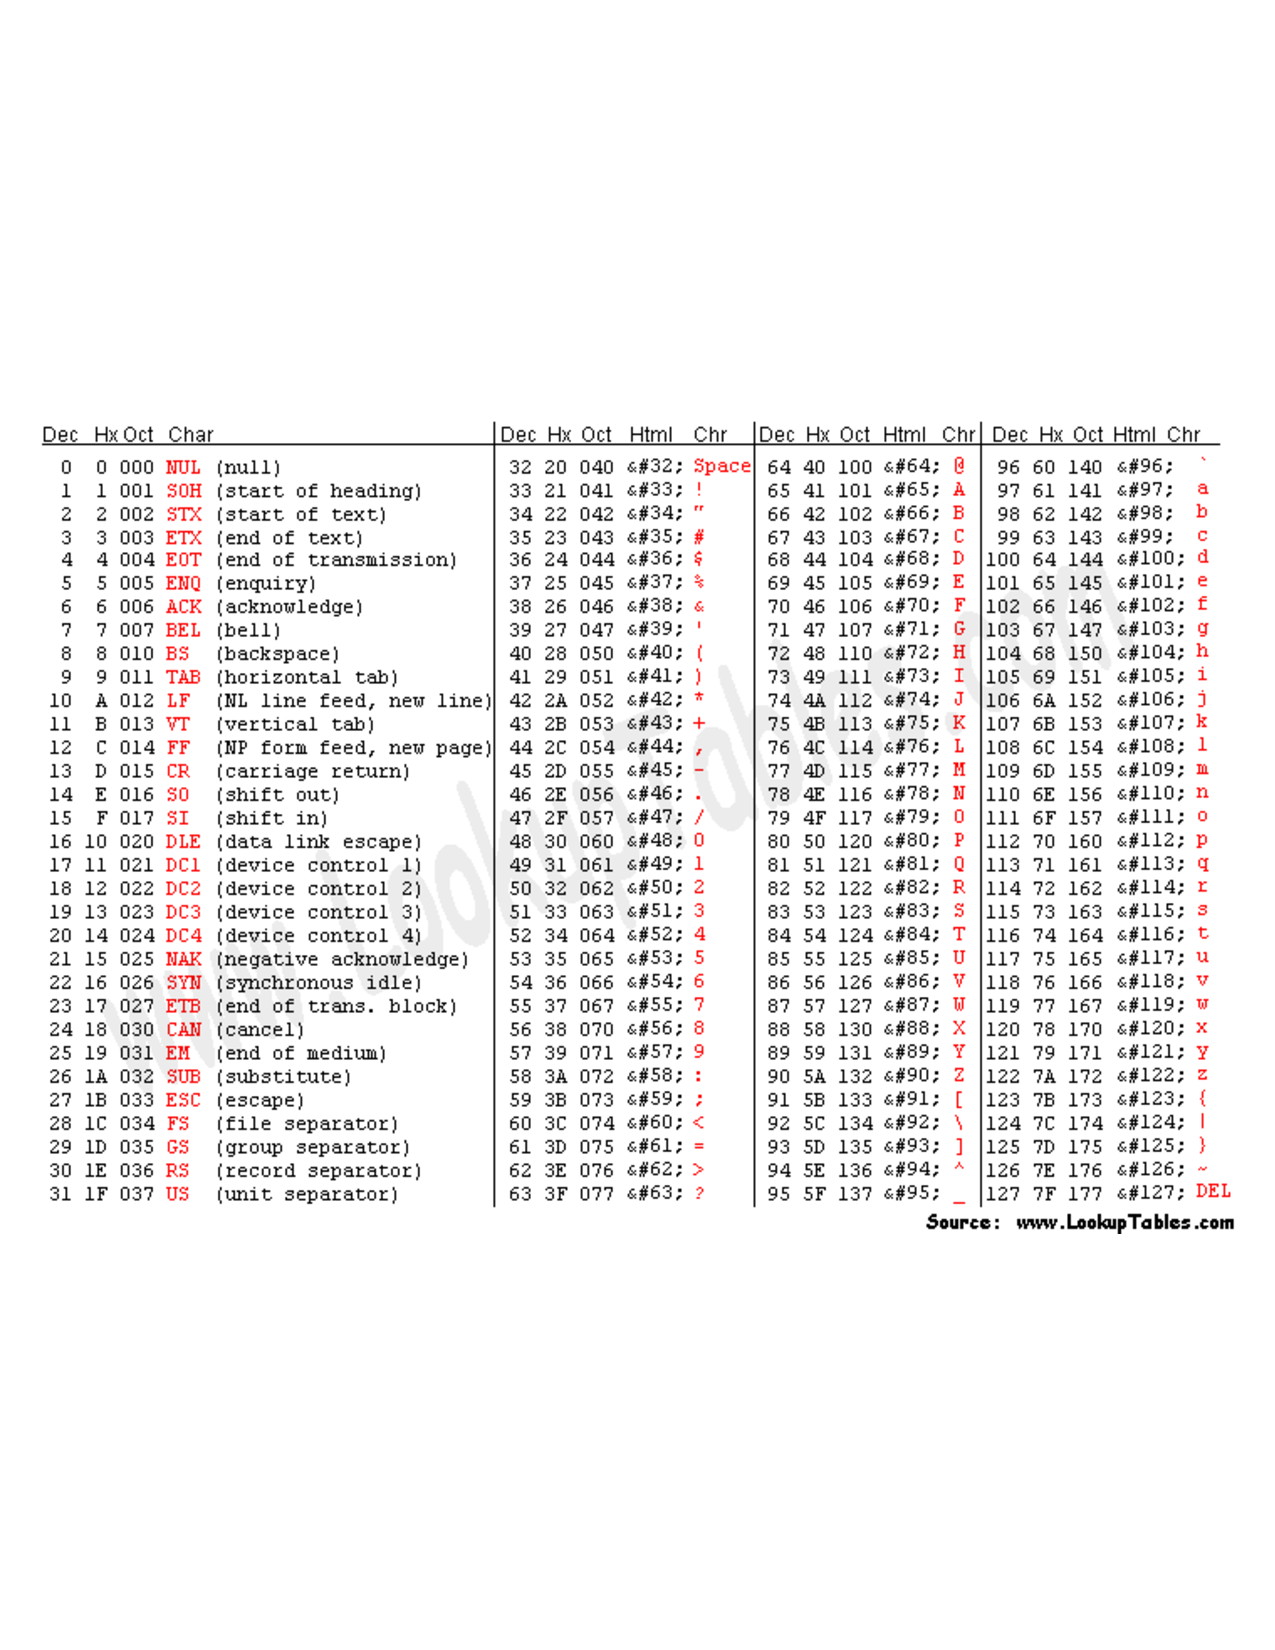
\includegraphics{figures/asciifull}}

You can think of this is kind of an encryption. Instead of saying ``Hi'' you might say ``73 105.''
 
There are multiple standards but the clear winner is \href{http://www.asciitable.com/}{ASCII}. In the old days there was also \href{http://www.lookuptables.com/ebcdic_scancodes.php}{EBCDIC}.

\scalebox{.55}{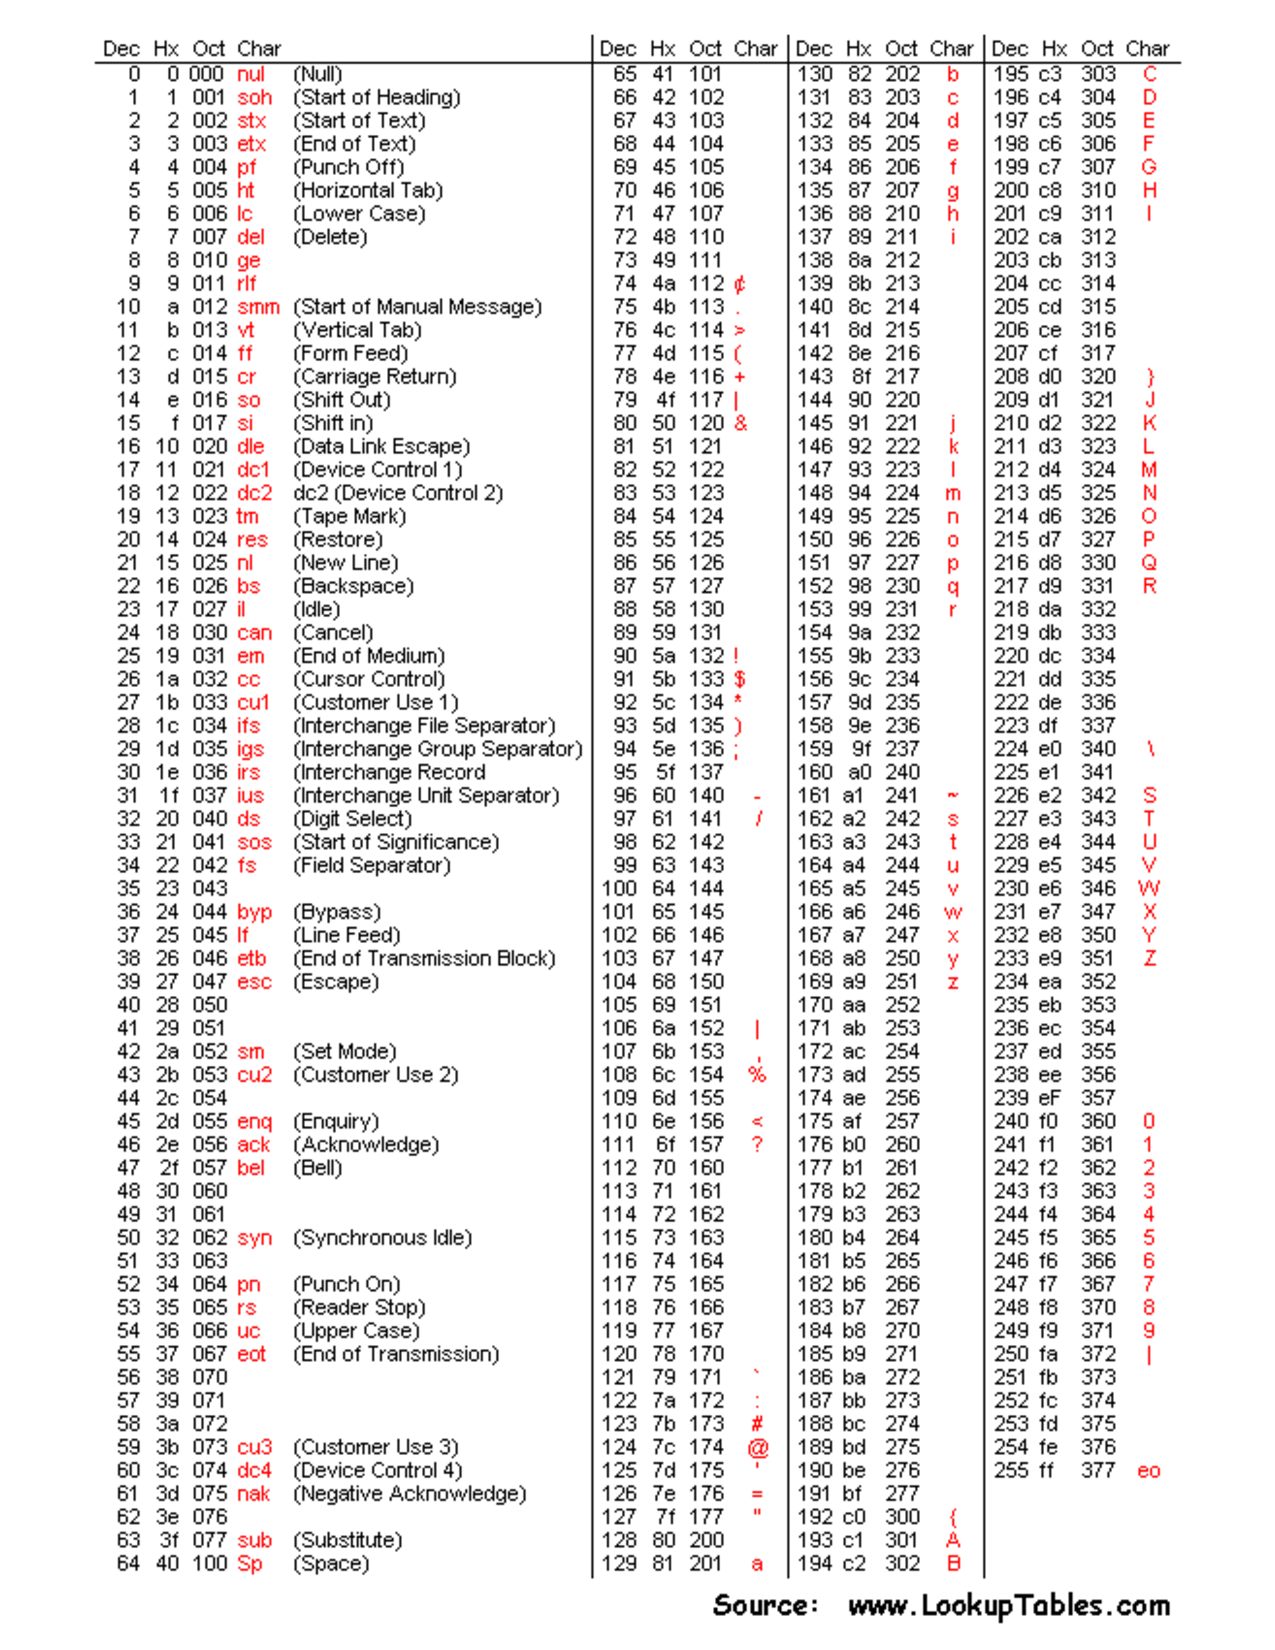
\includegraphics{figures/ebcdic}}

As we will see shortly, a phrase or sentence or word is just a sequence of characters hence a sequence of numbers stored in the machine.

\subsection{Images}

Images are stored as numbers also. Each pixel on the screen is typically represented by three numbers, it's red green and blue RGB values. For example 

white: 255 255 255  (yes they are one byte each) \\
black: 0 0 0\\
blue: 0 0 255 (blue is saturated)\\
Yellow is a mix of red and green: 255 255 0

Show omnigraffle were other application that will show color.

or, we can use a single bit to represent a black-and-white image where zero means off and one means on:

\scalebox{.15}{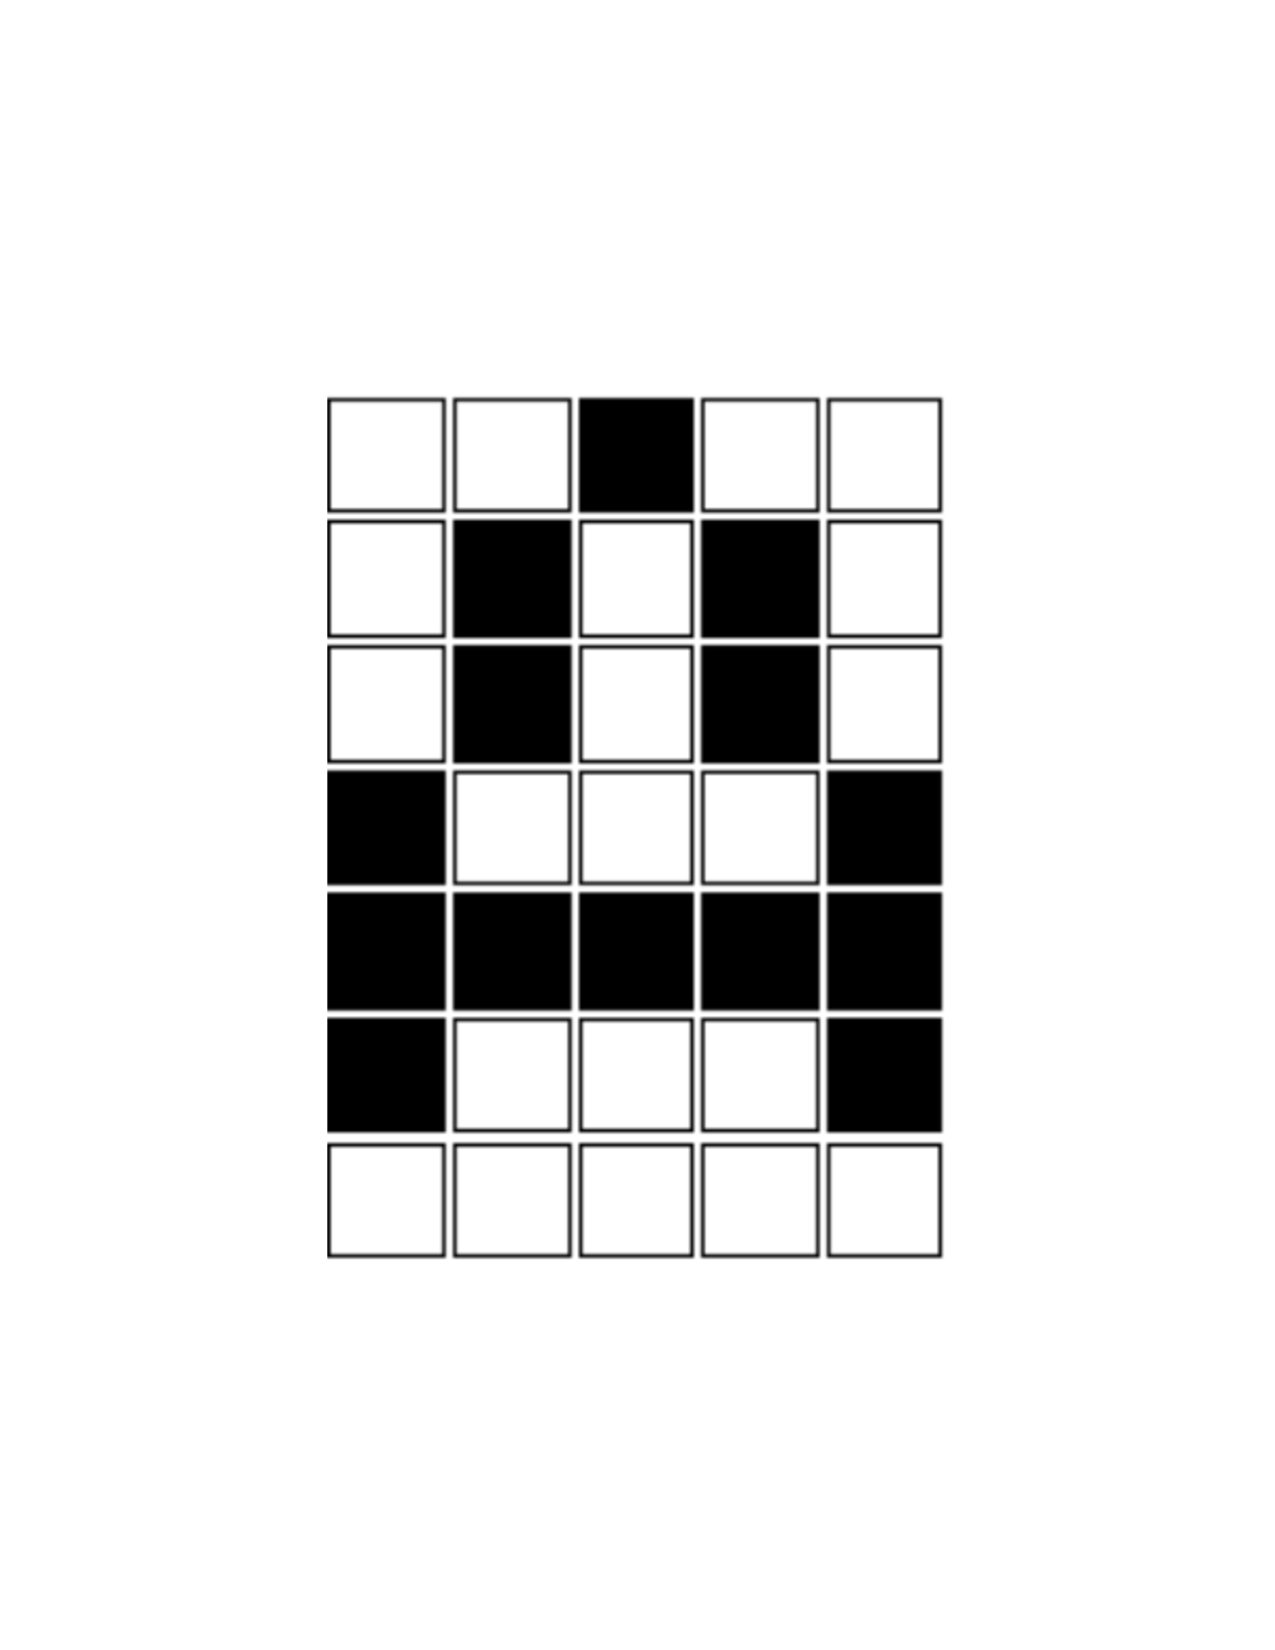
\includegraphics{figures/a-image}}

The bit sequence is:

{\tt 00100 01010 01010 10001 11111 10001 00000}

if you stack vertically, you can see the image sort of

{\tt 00100\\
     01010 \\
     01010 \\
     10001 \\
     11111 \\
     10001 \\
     00000}

\subsection{Audio}

From Wikipedia page on \href{https://en.wikipedia.org/wiki/Digital_audio}{Digital audio}:

\scalebox{.35}{\includegraphics{figures/waveform-quant.svg}}

\section{Atomic elements}

There are a few basic or atomic elements in Python and each kind of element knows not only its value but also its type. Is very important to learn the difference between value and type.

\subsection{Integers}

These are just numbers that were used for counting; whole numbers like -9, 0, 3, 1023023823. You can make these things you like
 
\begin{pyconsole}
type(323241321234123412348123091324)
\end{pyconsole}

but if they are smaller they go into a different type. {\tt type} just another function call that asks the type of something.

\begin{pyconsole}
type(3232)
\end{pyconsole}

\subsection{Real numbers}
 
Real numbers, not whole numbers, are of finite precision but can hold some very large and very small numbers.

\begin{pyconsole}
3.14159
0.000000000001
23e100
\end{pyconsole}

The {\tt e} stuff is the scientific notation and represents the exponent. We call these floating-point numbers.

\subsection{Boolean values}

A Boolean value is either true or false, but Python also allows a number of other things to represent true and false such as 1 can be true and 0 can be false.

\begin{pyconsole}
True
False
bool(1)
bool(0)
bool(36)
bool("hi")
\end{pyconsole}

\subsection{Strings}

Single, double, or triple quotes. 0 or more characters in between delimiters. We call these literals or hardcoded values.

\begin{pyconsole}
'a'  # a single character string is sometimes called a character
'hi'
"hi"
"""hi"""
\end{pyconsole}

When you need to actually include quotes of some kind in the string, then you surround it with different quotes like {\tt "Bob's house"}.

{\bf Exercise}: write a Python program to print out: {\tt My name is "Terence"}

\subsection{Special characters}

{\tt \textbackslash n}  is the newline character, {\tt \textbackslash t}  is the tab character


\begin{pyconsole}
print "Cars:\n\tBMW\n\tAudi"
\end{pyconsole}

which is the same thing as
 
\begin{pyconsole}
print "Cars:"
print "\tBMW"
print "\tAudi"
\end{pyconsole}

or

\begin{pyconsole}
print "Cars:"
print "	BMW"
print "	Audi"
\end{pyconsole}


\subsection{Conversions}

We can convert between numbers

\begin{pyconsole}
float(3)
int(3.14159)
\end{pyconsole}

and numbers and characters

\begin{pyconsole}
chr(100)
chr(105)
ord('H')
str(234)
\end{pyconsole}

\end{fullwidth}